%Dave's handout 6.5 (Average Value of a Function)

\vspace{-0.25 in}
\begin{framed}
\subsection*{Objectives}
\begin{itemize}
    \item Be able to apply the concept and techniques of definite integration to find \emph{Average Value of A Function}.
    \item Be able to find the \emph{Average Value of A Function} in different applications.
\end{itemize}

%%%Reading Assignment%%%
\subsection*{Suggested Reading:}
\begin{itemize}
\item \cite{Calaway}\footnotemark[1]
   \begin{itemize}
        \item \emph{Section 3.6 Area, Volume, and Average Value}
        \begin{itemize}
            \item Average Value
        \end{itemize}
    \end{itemize}
    
\item \cite{openstax}\footnotemark[2]\textsuperscript{,}\footnotemark[3]
    \begin{itemize}
        \item \emph{Section 5.2 The Definite Integral}
        \begin{itemize}
            \item Average Value of a Function
        \end{itemize}
    \end{itemize}
\end{itemize}
%\subsection*{Supplemental Materials:}
%%%Key Terms%%%
\subsection*{Key Terms and Concepts:} 

\begin{multicols}{2}
\begin{itemize}
    \item Average value of a function
    
\end{itemize}
\end{multicols}
\end{framed}
\footnotetext[1]{Available free to download from \url{http://www.opentextbookstore.com/details.php?id=14} .}
\footnotetext[2]{Available free to download from \url{https://openstax.org/details/books/calculus-volume-1} .}
\footnotetext[3]{Disregard any examples with trigonometry.}

\newpage
%%%%%%%%%%START LESSON CONTENT%%%%%%%%%%%%%
%\noindent\makebox[\linewidth]{\rule{\textwidth}{0.8pt}}
\Opensolutionfile{ans}[ans24]
\Opensolutionfile{ansL}[ansL24]
%%%%%%%%%%%%%%%%Start First Topic%%%%%%%%%%%%%%%%%%%%%%%%%%%%%
\noindent Suppose we are using an exponential growth model to predict the population, $P$, of a county at time $t$ years in the future: $P(t)=P_0e^{kt}$; $t\ge 0$.  Clearly, at any point in time, the population will be different from any previous or future point in time.  One question that may be asked is what the \textbf{average value} of the population would be over some particular time interval, say $t=a$ to $t=b$.\\

\noindent The concept of the average of a set of measurements is understood, that is the sum of $n$ numbers ($a_1, a_2,...,a_n$) is their sum divided by $n$. However, there are an infinite number of points in time, and hence an infinite number of values for the population size.  So we cannot sum up all of the population sizes and divide by the number of observations since there is an infinite number of each.  The key is to remember our previous approach using definite integrals to determine the area under the graph of a function, in which the sum of an infinite number of terms approached the value of a definite integral.  As such, we have the following method for determining the average value:  

\begin{tcolorbox}[title = {Average Value of A Function}]

\noindent Let $f(x)$ be continuous over the interval $[a,b]$. Then, the \textbf{average value of the function} $f(x)$ (or $\bm{f_{ave}}$) on $[a,b]$ is given by
\begin{equation}\label{eq:averageValueFn}
f_{ave}=\frac{1}{b-a}\int_a^b f(x)\,dx
\end{equation}

\end{tcolorbox}

%%%%%Geometric Interpretation from Calaway, Applied Calculus (page 210)
\begin{figure}[h!]
    \centering
    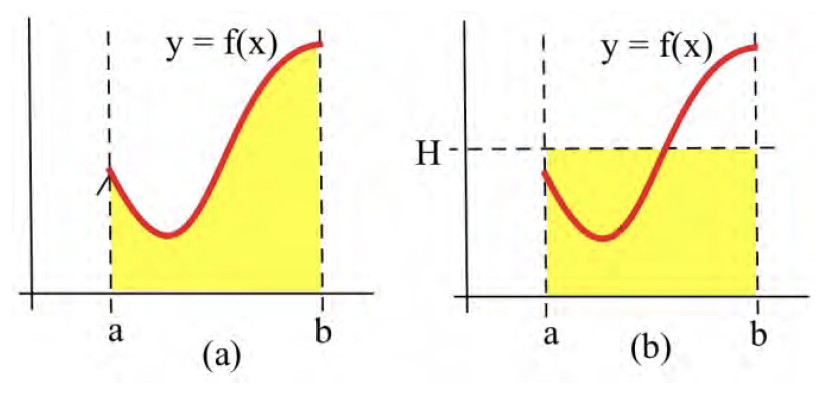
\includegraphics[scale=0.5]{images/defIntgApp/geometricInterpret.png}
    \caption{}
    \label{fig:geometricInterpret}
\end{figure}

\noindent The average value of a positive f has a nice geometric interpretation. Imagine that the area under $f$ (Figure \ref{fig:geometricInterpret} (a)) is a liquid that can "leak" through the graph to form a rectangle with the same area (Figure \ref{fig:geometricInterpret} (b)).\\

\noindent If the height of the rectangle is $H$, then the area of the rectangle is $H\cdot (b-a)$. We know the area of the rectangle is the same as the area under $f$ so $H\cdot (b-a)=\displaystyle\int_b^a f(x)\,dx$. Then $H=\displaystyle \frac{1}{b-a}\int_b^a f(x)\,dx$, the average value of $f$ on $[a,b]$. The average value of a positive function $f$ is the height $H$ of the rectangle whose area is the same as the area under $f$.
%%%Example 4 from 3.6 Calaway, Applied Calculus (page 211)%%%

\begin{example}
During a 9 hour work day, the production rate at time $t$ hours after the start of the shift was given by the function $r(t)=5+\sqrt{t}$ cars per hour. Find the average hourly production rate.
    %%short answer
    \begin{sol}
    $f_{ave}=\displaystyle\frac{1}{2}\cdot \left[50000e^{0.08x}\right]_0^2= 7$ cars per hour.
    \end{sol}
    %%solution
    \begin{solL}
    Complete solution here.....
    
    \end{solL}
    
\end{example}
\vspace*{\stretch{1}}
\newpage
\noindent \textbf{Look Back:} A note about the units – remember that the definite integral has units cars per hour $\times$ hours = cars. But the $\displaystyle\frac{1}{b-a}$ in front has units 1/hours – the units of the average value are cars per hour, just what we expect an average rate to be. \textbf{In general, the average value of a function will have the same units as the integrand.}

%%%Examples%%%
\begin{example}
After an aggressive campaign to lure high-tech industries, a county with a current population of 10,000 people is expected to see an increase in population over the next 20 years.  The county planning commission is using an exponential growth model to predict the population size at time t years from the present: $P(t)=10000e^{0.08t}$; $0\le t \le 20$ (Note:  An annual growth rate of 8\% compounded continuously.) 
\renewcommand{\labelenumi}{\textbf{(\alph{enumi})}}
    \begin{enumerate}[leftmargin=*]
    \item Find $P(0)$ and $P(5)$. Interpret the results.\vspace*{\stretch{0.6}}
    \item Determine the predicted average population of the county over the next 5 years. Round to the nearest whole number.\vspace*{\stretch{1.5}}
    
    \item 	Determine the predicted average population of the county over the interval from $t=10$ years to $t=15$ years. \vspace*{\stretch{1}}
    \end{enumerate}
    %%short answer
    \begin{sol}
    \renewcommand{\labelenumi}{\textbf{(\alph{enumi})}}
    \begin{enumerate}[leftmargin=*]
    \item The current population size is $P(0)=10000$ people; the population size after 5 years (at time $t=5$) is $P(5)\approx 14,918$ people
    \item $f_{ave}=25000e^{0.08t}\Big|_0^5\approx 12,296$ people.
    \item $f_{ave}=25000e^{0.08t}\Big|_{10}^{15}\approx 27,364$ people.
    \end{enumerate}
    \end{sol}
    %%solution
    \begin{solL}
    Complete solution here.....
    
    \end{solL}
    
\end{example}
%\vspace*{\fill}
\newpage
\noindent \textbf{Look Back:} Exponential Growth means that the population will grow at a faster rate as time goes on: $P'(t)=k\cdot P(t)$. These are both 5-year intervals but the average value is greater for the $2^{nd}$ interval as the population continues to increase. DO NOT confuse \underline{\textbf{rate}} and \underline{\textbf{average}}.\\

\noindent \textbf{Extra Note:}\\

\noindent Function averages, involving means and more complicated averages, are used to "\emph{smooth}" data so that underlying patterns are more obvious and to remove high frequency "\emph{noise}" from signals. In these situations, the original function $f$ is replaced by some "average of $f$." If $f$ is rather jagged time data, then the ten year average of $f$ is the integral $g(x)=\displaystyle\frac{1}{10}\int_{x-5}^{x+5} f(t)\, dt$, an average of $f$ over 5 units on each side of $x$. For example, the figure \ref{fig:temperature}  shows the graphs of a Monthly Average (rather “\emph{noise}” data) of surface temperature data, an Annual Average (still rather “\emph{jagged}"), and a Five Year Average (a much smoother function). Typically the average function reveals the pattern much more clearly than the original data. This use of a “\emph{moving average}” value of “\emph{noisy}” data (weather information, stock prices) is a very common.
\begin{figure}[h!]
    \centering
    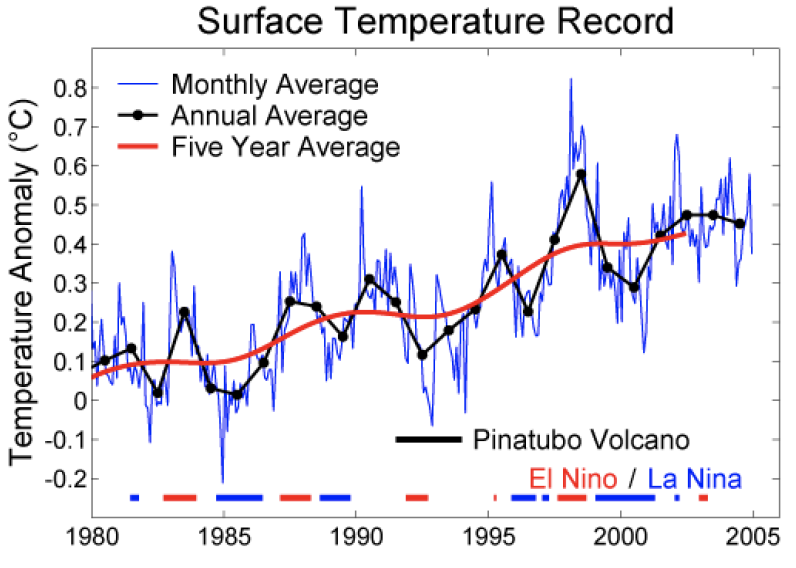
\includegraphics[scale=0.8]{images/defIntgApp/temperature.png}
    \caption{}
    \label{fig:temperature}
\end{figure}
%%%%%%%Add a real-world example: "Surface Temperature Record" example from Calaway, Applie Calculus (page 211)

%%%%%%%%%%%%End Examples%%%%%%%%%%%%%%%%%%
%%%%%%%%%%%%%%%End Topic%%%%%%%%%%%%%%%%%%



%%%%%%%%%%%%%%%End Lesson%%%%%%%%%%%%%%%%%%
\Closesolutionfile{ans}
\Closesolutionfile{ansL}

%%%Short Answers to Examples%%%


\vspace*{\fill}
\subsection*{Short Answers to Examples}
%\vspace{-0.25cm}

%\begin{multicols}{2}
\input{ans24}
%\end{multicols}



